\section{Internet of Things}
\ac{IoT} steht für die Vernetzung von Gegenständen, die primär keine Rechner sind. \ac{IoT} ist in der Literatur nicht scharf definiert. Der wissenschaftliche Mitarbeiter des MITs Kevin Ashton hat sich 1999 wie folgt zum Thema \ac{IoT} geäußert: 
\begin{quote}
If we had computers that knew everything there was to know about things -- using data they gathered 
without any help from us -- we would be able to track and count everything, and greatly reduce waste, 
loss and cost. We would know when things needed replacing, repairing or recalling, and whether they 
were fresh or past their best. We need to empower computers with their own means of gathering 
information, so they can see, hear and smell the world for themselves, in all its random glory. RFID and 
sensor technology enable computers to observe, identify and understand the world—without the 
limitations of human-entered data.
\end{quote}

Der Hintergedanke bei den meisten Definitionen von \textit{\ac{IoT}} ist, Abläufe zu automatisieren. Damit die \textit{Things}, die \ac{IoT}-Geräte, nützlich sein können, müssen sie ihre Umwelt wahrnehmen können. Dazu kommen Technologien wie 
\begin{itemize}
\item \ac{RFID}
\item \ac{NFC}
\item und Bluetooth
\end{itemize} 
zum Einsatz.
Die eigentliche Idee dazu, entwickelte sich nicht erst in den letzten Jahren. Die Umsetzung der Idee ist jedoch begünstigt durch Fortschritte bei der Entwicklung von Batterien und Akkumulatoren, kompakten Photovoltaikelementen und mobilen Datennetzen (LTE, UMTS). 
Damit in Zukunft viele Geräte im Internet kommunizieren können, ist man auf lange Sicht wahrscheinlich dazu gezwungen, das Internetprotokoll Version sechs zu verwenden. Das Internetprotokoll in der Version vier unterstützt in der Theorie nur zirka 4,3 Milliarden ($2^{32}$) Geräte. Durch die Nutzung von Verfahren wie Network Adress Translation (NAT) geht man momentan noch Enpässen bei der Vergabe von Adressen aus dem Weg. 

\begin{figure}
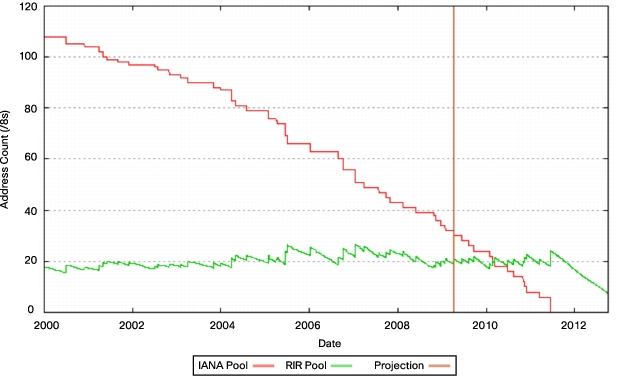
\includegraphics[scale=0.7]{bilder/ipv4cisco} 
\caption[Verfügbarkeit von IPv4 Adressen bei den beiden IP-Vergabeorganisationen IANA und RIR ]{Verfügbarkeit von IPv4 Adressen bei den beiden IP-Vergabeorganisationen IANA und RIR \cite{cisco}}
\label{IPv4}
\end{figure}


Um nun aber mehr als zirka 4,3 Milliarden Geräte direkt zu adressieren, muss man ein anderes Protokoll verwenden. Hier bietet sich das Internetprotokoll Version 6 an. Die Adressen sind nun nicht mehr nur 32 Bit lang, sondern 128 Bit. Das ermöglicht eine Adressierung von $2^{128}$ Geräten. So könnte man ohne Engpässe alle IoT-Geräte direkt adressieren. 
Eine wichtige Rolle im Hinblick auf IoT ist die Maschine-zu-Maschine-Kommunikation. Für die Realisierung dieser ist es essentiell, dass jede Maschine (IoT-Gerät) erreichbar und eindeutig adressierbar ist. Die Nutzung des Internetprotokolls in der Version sechs kann dies sicherstellen. Die Maschine-zu-Maschine-Kommunikation wird in diesem Kapitel noch genauer betrachtet.     
Ferner hat IoT der Definition der Firma Lopez Research nach folgende Paradigmen:
\begin{itemize}
\item Kommunikation
\item Kontrolle
\item Kostensenkung
\end{itemize} 
\textit{Kommunikation} meint, was oben schon beschrieben ist. Die Kommunikation ist für Iot-Geräte essentiell. \textit{Kontrolle} meint, dass IoT die Möglichkeit bieten soll, dass ein Benutzer jeder Zeit ein IoT-Gerät kontrollieren kann. Ein Beispiel könnte sein, dass man die Waschmaschine von unterwegs mit Hilfe des Smartphones aktivieren kann. 

\cite{cisco}
